\def\relativepath{BiPart/} % ← chemin relatif depuis le main

\graphicspath{{\relativepath Figures/}} % pour les images
\makeatletter
\def\inputfile#1{\input{\relativepath#1}} % pour les sous-fichiers
\makeatother

\makeatletter
\let\oldinput\input
\def\input#1{\oldinput{\relativepath#1}}
\makeatother

% Utilisation :
%\inputfile{texte.tex}
%\includegraphics[width=\textwidth]{image1.png}



%\chapter{Quench bipartite dans un gaz de Bose unidimensionnel}

\section*{Introduction}

Dans ce chapitre, nous étudions l’évolution d’un gaz quantique unidimensionnel après une rupture de symétrie initiale. Nous utilisons un gaz de bosons ultra-froids, confiné dans une géométrie unidimensionnelle. Ce gaz est bien décrit par le modèle intégrable de Lieb-Liniger. Les interactions entre atomes sont courtes et répulsives.

Nous préparons d’abord un gaz homogène (Fig \ref{fig:BiPart.insitut}). Ensuite, nous supprimons brutalement une moitié du nuage. Cela crée une frontière nette entre deux zones : une avec des atomes, l’autre vide. Cette configuration correspond à ce qu’on appelle un « quench bipartite ».

\begin{figure}[H]
	\centering
	\includegraphics[width=0.5\textwidth , page = 4 ]{Shema.pdf}
	\caption{a) Facteur d'occupation initial $\nu(x, \theta) = \nu_0(\theta)$ correspondant à l'équilibre thermique à la température $T = 560~\mathrm{nK}$, pour une densité spatiale linéique $n_p = 56~\mu\mathrm{m}^{-1}$, soit une potentielle chimique $\mu = 65~\mathrm{nK}$.  
b) Densité spatiale linéique $n(x) = \int \rho_{[\nu]}(x, \theta)\, d\theta \equiv n_p = 56~\mu\mathrm{m}^{-1}$.  
c) Facteur d'occupation initial $\nu_0(\theta)$ correspondant au cas présenté en a).}
	\label{fig:BiPart.insitut}
\end{figure}


\begin{figure}[H]
	\centering
	\begin{subfigure}[b]{0.3\textwidth}
		\begin{tikzpicture}
			\begin{scope}[shift={(2,0)}]
				\begin{scope}[transform canvas={scale=0.6}]
					%\input{Figures/Fonc_A_code}	
			
				\end{scope}
			
				\draw[color = red , scale = 0.5 , draw = none  ] (-2 , -1) rectangle (5, 6) ; 	
			\end{scope}
					
		\end{tikzpicture}
		\caption{}
		\label{fig:grap.A}
	\end{subfigure}
	\hfill
	\begin{subfigure}[b]{0.65\textwidth}
		\begin{tikzpicture}

			\begin{scope}[shift={(-11,2.7)}]
				\begin{scope}[transform canvas={scale=0.6}]
					%% Définition des couleurs avec les codes HTML
\definecolor{colorOne}{HTML}{443E46}
\definecolor{colorTwo}{HTML}{F6DEB8}
\definecolor{colorThree}{HTML}{908CA4}
\definecolor{colorFour}{HTML}{57659E}
\definecolor{colorFive}{HTML}{C57284}
\definecolor{colorSix}{HTML}{FF5B69}

% Raccourcis pour les couleurs
\def\colorOne{colorOne}
\def\colorTwo{colorTwo}
\def\colorThree{colorThree}
\def\colorFour{colorFour}
\def\colorFive{colorFive}
\def\colorSix{colorSix}

\def\colorslide{blue!50!black}

\def\Occupation{
	\def\traitx{0.3}
	\def\traity{0.5}
	\draw[shift={(0,0)}]
		(-13.5 , 0 ) edge [thick,line width=0.8ex ]( -3.2  , 0 )
		( -3.2 - \traitx  , 0 - \traity ) edge [thick,line width=0.8ex ]( -3.2 + \traitx  , 0 + \traity  )
		( -2.8 - \traitx  , 0 - \traity ) edge [thick,line width=0.8ex ]( -2.8 + \traitx  , 0 + \traity  )
		(-2.8 , 0 ) edge [thick,line width=0.8ex ](2.8  , 0 )
		( 2.8 - \traitx  , 0 - \traity ) edge [thick,line width=0.8ex ]( 2.8 + \traitx  , 0 + \traity  )
		( 3.2 - \traitx  , 0 - \traity ) edge [thick,line width=0.8ex ]( 3.2 + \traitx  , 0 + \traity  )
		(3.2, 0 ) edge [thick,line width=0.8ex,->,>=triangle 45 , color = black ]node [pos=1.01,below  ]{\huge$\theta$}	( 13  , 0 )
	;
	\draw[shift={(0,0)}, color=\colorOne]
		(-10.5 , -1.5 ) edge [thick,line width=0.8ex , ->,>=triangle 45  ]( -10.5  , 4.5 )
	;
		
	\foreach \r in {1 , ... , 3 } {
%		\draw[
%		decoration={
%		markings,
%    	mark connection node=my node,
%    	mark=at position 0 with{\node [blue,transform shape] (my node) {\large \r};}},
%		color=gray, thick, 
%		line width=0.5ex] decorate { 
%            (-11.0, \r) -- (-10.1, \r )}
%        ;
        \draw[
			color=\colorOne,
			] 
            (-11.0, \r) edge[color=\colorThree , thick,line width=0.5ex] node [pos=-0.5 ]{\large\color{\colorFour} $\frac{\r}{\delta \theta}$ } (-10.3, \r )
        	;
	
	}
	

	
	% Graduation abcsisse 
	% Définitions des listes
% Definitions of the lists
\def\listetuple{-9/\theta_{1}, -8/\theta_{2} , -5/\theta_{3} , -2/\theta_{a-1} , 0/\theta_{a} , 1/\theta_{a+1} , 2/\theta_{a+2} ,  5/\theta_{N-4} , 7/\theta_{N-3},8/\theta_{N-1},9/\theta_{N} }
\def\listetrais{-12 , -11, -10, -9 , -8 , -7 ,  -6 , -5, -4.5,-4, -2 , -1, 0 , 0.5, 1, 2, 4 , 5 ,  6 , 7 , 8 ,8.5, 9 ,  10 , 11, 12 }

% Loop over listetrais
\foreach \r in \listetrais {
    % Initialize found variable to zero
    % Initialize found variable to zero
    %\pgfmathsetmacro\found{0}
    \global\def\found{0}
    \xdef\nomtheta{}
    
    % Check if \r is in listetuple
    \foreach \x/\y in \listetuple { 
        \ifdim \r pt=\x pt % If \r matches any \x in listetuple
            \global\def\found{1} ;
            \xdef\nomtheta{\y} % Set \nomtheta to the corresponding \y
            %\pgfmathsetmacro\found{1} % Set found to 1            
            %\global\pgfmathsetmacro\found{1}
        \fi
    }
    
    %\node [circle, draw, red] (A) at (\r, 2) {\found , $\nomtheta$};
    
    % Draw the line and display \nomtheta if found
    \ifnum\found=1
        \draw[color=\colorOne, thick, line width=0.5ex] 
            (\r, -0.3) -- (\r, 0.3) node[red , pos=-0.5] {\large $\nomtheta$};
         \filldraw[line width=0.5ex, color=\colorSix, outer color=\colorSix, inner color=\colorSix] 
            (\r, 0) circle (4pt);
    \else 
        % Draw without \nomtheta and add a blue circle if not found
        \draw[color=\colorOne, thick, line width=0.5ex] 
            (\r, -0.3) -- (\r, 0.3);
        \filldraw[line width=0.5ex, color=\colorSix, outer color=\colorTwo, inner color=\colorTwo] 
            (\r, 0) circle (4pt); 
    \fi
}

\def\listetrais{-9.5/\theta_{i-1}/2/3, -6.5/\theta_{i}/1/4  ,   -1.5/\theta_{j}/2/4 , 1.5/\theta_{j+1}/-1/3 , 3.5/\theta_{\ell-1}/1/3 , 6.5/\theta_{\ell}/3/4 , 9.5/\theta(\theta_{\ell+1})/-1/3 };



\foreach \r/\nomx/\y/\ys in \listetrais {
	\draw[
		decoration={
		markings,
    	mark connection node=my node,
    	mark=at position .5 with{\node [blue,transform shape] (my node) {\large \color{\colorFour} $\nomx$};}},
		color=\colorThree , thick, 
		line width=0.5ex] decorate { 
            (\r, 0.12) -- (\r, -1.2)}
        ;
     
     \ifdim \y pt > -1 pt 
     	\draw[
			decoration={
			markings,
    		mark connection node=my node,
    		mark=at position .5 with{\node [blue,transform shape] (my node) {\large \color{\colorFour} $\pi^d(\nomx) $};}},
			color=\colorThree, thick, 
			line width=0.5ex] decorate { 
            (\r, \y) -- (\r +3, \y)}
        ;
        \draw[
			decoration={
			markings,
    		mark connection node=my node,
    		mark=at position .5 with{\node [blue,transform shape] (my node) {\large \color{\colorFive} $\pi_s^d(\nomx) $};}},
			color=\colorFive, thick, 
			line width=0.5ex] decorate { 
            (\r, \ys) -- (\r +3, \ys)}
        ;
     \fi 
     \ifdim \r pt= -1.5 pt
     	\draw[
     		decoration={
			markings,
    		mark connection node=my node,
    		mark=at position .5 with{\node [blue,transform shape] (my node) {\large \color{\colorFour}  $\delta \theta $};},
    		%mark=at position 0.1  with {\arrow[blue, line width=0.5ex]{<}},
    		%mark=at position 1  with {\arrow[blue, line width=0.5ex]{>}}
    		},
        	color=\colorThree,
        	thick,
        	line width=0.5ex,
        	%arrows={Computer Modern Rightarrow[line cap=round]-Computer Modern Rightarrow[line cap=round]}
   			](\r, -1.2) edge[arrows={Computer Modern Rightarrow[line cap=round]-}] (\r + 0.4, -1.2)decorate {
    		(\r, -1.2) -- (\r + 3, -1.2)}(\r + 2, -1.2) edge[arrows={-Computer Modern Rightarrow[line cap=round]}] (\r + 3, -1.2)
    		;
    \fi
			
	
}


			
}


\begin{scope}
	%\draw[help lines , width=1.5ex] (-8,-3) grid (8,3);\draw[help lines ,width=0.5ex , opacity = 0.5] (-3,-3) grid[step=0.1] (3,3));
	
	%\draw[help lines] 
	%	(-3,-3) edge[width=1.5ex] grid (3,3)	
	%	(-3,-3) edge[width=0.5ex , opacity = 0.5] grid (3,3)	
	%;
	\begin{scope}[shift={(0,1)},rotate=0,opacity=1,color=black]
		\Occupation	
		
		%\node[anchor=east, font=\bfseries] at (-11, 0) {\color{red}\large (T = 0 )} ;	
	\end{scope}
	
	
	
	
	\begin{scope}[shift={(-10.5,7)},rotate=0,opacity=1,color=black]
	
	\begin{scope}[shift={(-0,0)},rotate=0,opacity=1,color=black]
	
		\draw[shift={(0,0)} ,line width=1ex,rounded corners = 1ex,color=\colorOne , opacity =1 ,fill=\colorOne!00 , pattern={north east lines} , pattern color=\colorOne!00 ]
			(0 , -1 ) rectangle (5,1)
		;
		

		\begin{scope}[shift={(0.5,0.5)}]
			\draw[color=\colorOne, thick, line width=0.5ex] 
            (0, -0.3) -- (0, 0.3) ;
            \filldraw[line width=0.5ex, color=\colorSix, outer color=\colorSix, inner color=\colorSix] 
            (0, 0) circle (4pt);
            
            \node[anchor=west, font=\bfseries] at (0.2, 0) {\color{\colorSix}\large : quasi-particule};
		\end{scope}
		
		\begin{scope}[shift={(0.5,-0.5)}]
			\draw[color=\colorOne, thick, line width=0.5ex] 
            (0, -0.3) -- (0, 0.3) ;
            \filldraw[line width=0.5ex, color=\colorSix, outer color=\colorTwo, inner color=\colorTwo] 
            (0, 0) circle (4pt);
            
            \node[anchor=west, font=\bfseries] at (0.2, 0) {\color{\colorSix}\large : hole};
		\end{scope}

	\end{scope}
	
	\begin{scope}[shift={(6,0)},rotate=0,opacity=1,color=black]	
		
		\draw[shift={(0,0)} ,line width=1ex,rounded corners = 1ex,color=\colorOne , opacity =1 ,fill=\colorOne!00 , pattern={north east lines} , pattern color=\colorOne!00 ]
			(0 , -1 ) rectangle (7.5,1)
		;
		
		\node[anchor=west] at (0.5, 0.5) {\color{\colorFour}\large $\pi^d$ };\node[anchor=west, font=\bfseries] at (0.9, 0.5) {\color{\colorFour}\large : quasi-particule distribution};
		
		\node[anchor=west] at (0.5, -0.5) {\color{\colorFour}\large $\pi_h^d$ };\node[anchor=west, font=\bfseries] at (0.9, -0.5) {\color{\colorFour}\large  : hole distribution};
		
	\end{scope}
	
	\begin{scope}[shift={(14.5,0)},rotate=0,opacity=1,color=black]	
		
		\draw[shift={(0,0)} ,line width=1ex,rounded corners = 1ex,color=\colorOne , opacity =1 ,fill=\colorOne!00 , pattern={north east lines} , pattern color=\colorOne!00 ]
			(0 , -0.5 ) rectangle (7.0,0.5)
		;
		
		\node[anchor=west] at (0.5, 0) {\color{\colorFour}\large ${\color{\colorFive}\pi_s^d} = \pi^d + \pi_h^d $ };\node[anchor=west, font=\bfseries] at (2.9, 0) {\color{\colorFour}\large {\color{\colorFive} : density of states}};
		
	\end{scope}
	
	
	\end{scope}


		
	
\end{scope}

	
			
				\end{scope}
				\begin{scope}[scale=1]
					\draw[color = red , scale = 1 , draw = none  ] (-1 , -1) rectangle (5, 5) ; 
				\end{scope}	
			\end{scope}
			
		\end{tikzpicture}
		\caption{}
		\label{fig.fluctu.A}
	\end{subfigure}
	\caption{}
	\label{fig:diag_fig}
\end{figure}


Le gaz évolue ensuite selon la dynamique de son Hamiltonien. Nous observons le déplacement de la frontière au cours du temps. Pour cela, nous mesurons le profil de densité atomique à différents temps d’évolution.

Nous voyons que la frontière se propage de manière balistique. La largeur du profil de densité augmente de façon linéaire avec le temps. Ce comportement est prédit par la théorie de l’hydrodynamique généralisée (GHD). Cette théorie décrit comment les propriétés locales d’un système intégrable évoluent dans le temps. %Elle repose sur une distribution appelée « distribution de rapidité ». Cette fonction décrit la répartition des quasi-particules dans le système.

Dans notre cas, GHD prévoit un profil de densité particulier si le gaz initial est à température nulle. Les données expérimentales sont proches de cette prédiction, mais avec de légers écarts. Ces écarts peuvent venir de la température non nulle du gaz ou d’autres imperfections expérimentales.

Nous montrons que le profil de densité contient beaucoup d’informations. En théorie, on peut retrouver la distribution de rapidité initiale à partir du profil de frontière. Cela permettrait d’avoir une méthode d’analyse très puissante, comme une sorte de « thermomètre généralisé ». %Cependant, cette méthode est sensible au bruit dans les données, surtout dans les parties du profil où la densité est très faible. Pour contourner cela, nous utilisons un modèle simple avec trois paramètres pour approximer la distribution de rapidité. Ce modèle donne de bons résultats et reste plus robuste.

Enfin, nous utilisons une nouvelle méthode expérimentale pour mesurer la distribution de rapidité localement {??} , à l’intérieur du profil. Nous observons une asymétrie, comme prévu par la théorie. D’un côté, la distribution est lisse et large ; de l’autre, elle est plus abrupte, comme pour un état fondamental. Cette observation confirme le comportement prédictif de la GHD, bien que la résolution spatiale limite la finesse des détails que nous pouvons observer.


\section{Dispositif expérimental}

Nous utilisons une puce atomique pour produire un gaz ultra-froid d’atomes de rubidium 87. (cf {??}) Les atomes sont dans l’état étiré $|F=2, m_F=2\rangle$. Un champ magnétique longitudinal uniforme de $B_0 = 3{,}36$ G est appliqué.

%Le piégeage transverse est assuré par trois microfils parallèles déposés sur la puce. Ces fils portent des courants alternatifs modulés à $400$ MHz. Cette configuration supprime les défauts dus à la rugosité des fils. Elle permet aussi de contrôler indépendamment les confinements longitudinal et transverse~\cite{PhysRevLett.98.263201}.

%Les atomes sont piégés à $7\,\mu$m de la surface de la puce et à $15\,\mu$m des fils. Cela donne un confinement transverse fort. Ce potentiel transverse est bien décrit par un piège harmonique. Sa fréquence est $\omega_\perp/2\pi = 2{,}56$ kHz pour les données présentées ici.

Par évaporation radiofréquence, nous refroidissons le gaz jusqu'à une température de $T = 100$ nK. Le potentiel chimique est $\mu/k_B = 45$ nK. Ainsi, on a $\mu/(\hbar\omega_\perp) = 0{,}4$ et $k_B T/(\hbar\omega_\perp) = 0{,}8$. Le gaz entre alors dans le régime unidimensionnel.

Le couplage effectif en 1D est donné par $g = 2 a_{3D} \hbar \omega_\perp$~(??), avec $a_{3D} = 5.3$~ nm, la longueur de diffusion en 3D pour le rubidium 87~(cf {??}).Le paramètre sans dimension de Lieb est $\gamma = mg / (\hbar^2 n_0)$, avec $n_0$ la densité linéaire. Il varie entre $0{,}004$ et $0{,}007$. La température vérifie $T \ll n_0^{3/2} \sqrt{\hbar^2 g / m}/k_B$, ce qui place le gaz dans le régime de quasi-condensat~(cf {??}).

Le piégeage longitudinal est assuré par quatre fils supplémentaires. Ces fils sont placés de part et d’autre des trois microfils transverses (voir Fig.~??(a)). Ils sont éloignés du centre de la puce. Le potentiel longitudinal est alors bien approché par une série de polynômes : $V(x) = \sum_i a_i x^i$.Nous ajustons les courants dans ces fils pour annuler les termes linéaire, quadratique et cubique ($a_1$, $a_2$, $a_3$). Le terme dominant est alors le terme quartique : $V(x) = a_4 x^4$.Ce type de piège crée une densité atomique quasi homogène sur une grande longueur. C’est important pour notre étude, car le protocole de coupure bipartite suppose un système semi-infini.Un exemple de profil de densité dans un tel potentiel est donné en gris sur la Fig.~\ref{fig:setup}(b). La densité linéaire $n_0$ reste constante à $10\%$ près sur une longueur d’environ $250\,\mu$m.

Pour créer la coupure initiale, nous utilisons une méthode de sélection spatiale~(cf {??}). %Nous éclaireons le bord gauche du nuage avec un faisceau quasi résonant. Ce faisceau est proche de la transition $F=2 \rightarrow F'=3$ de la raie D2. Il est perpendiculaire à l’axe longitudinal $x$.Les atomes exposés à ce faisceau subissent une pression de radiation. Une exposition de $30\,\mu$s (environ 15 cycles d’absorption/réémission) suffit pour qu’ils quittent le piège. Le faisceau est façonné à l’aide d’un dispositif à micro-miroirs (DMD) pour ne viser qu’un bord du gaz.

Cette méthode crée une frontière nette entre une région vide et un gaz homogène. Cette netteté est surtout limitée par la résolution de l’image, de l’ordre du micromètre. L’effet de réabsorption des photons diffusés peut aussi réduire la netteté. Pour l’atténuer, on détune le faisceau de $15$ MHz par rapport à la transition D2.

Le profil de densité après cette sélection est montré en jaune dans la Fig.~\ref{fig:setup}(b). Le gaz est alors homogène à $10\%$ près sur environ $200\,\mu$m.

Après cette préparation, nous relâchons le confinement longitudinal tout en maintenant le piège transverse. La frontière initiale s’élargit avec le temps. Nous suivons cette dynamique en enregistrant les profils de densité $n(x,t)$ à différents temps d’évolution.

\section{Prédictions de la GHD}\label{sec.GHDpredictions}
\label{sec:ghd}

Le dispositif expérimental décrit ci-dessus peut être analysé théoriquement comme suit. Au cours de l'évolution temporelle, la frontière nette initiale du nuage devient plus lisse et les dérivées temporelles des quantités locales diminuent. Après un certain temps, après un lissage, on s'attend à ce que le gaz puisse être décrit localement par des états stationnaires.

Les états stationnaires du modèle de Lieb-Liniger sont complètement caractérisés par leur distribution de rapidité $\rho(\theta)$. Alternativement, ces états peuvent être caractérisés par une fonction $\nu(\theta)$ appelée "facteur d'occupation".% qui prend des valeurs entre 0 et 1, et qui est liée à la distribution de rapidité $\rho(\theta)$ par
%\begin{equation}
%\nu(\theta) = \frac{\rho(\theta)}{\rho_s(\theta)} \mbox{, \qquad où \qquad } \rho_s(\theta) =
%\frac{m}{2\pi \hbar} + \int \frac{d\theta'}{2\pi} \Delta(\theta-\theta') \rho(\theta') ,
%\end{equation}
%et $\Delta(\Theta) = \frac{2g}{\left(\frac{g^2}{\hbar} + \hbar \Theta^2\right)}$ est le "décalage de diffusion" dans le modèle de Lieb-Liniger. Les fonctions $\nu$ et $\rho$ sont en correspondance biunivoque, et dans ce qui suit, nous utilisons alternativement $\rho$ ou $\nu$. [Pour une introduction à ce formalisme, nous nous référons aux notes de cours \cite{doyon2020lecture} ou à la Section 1 de l'article de revue \cite{bouchoule_generalized_2022}.]

Puisque nous supposons une stationnarité locale, le système dans son ensemble est décrit par une distribution de rapidité dépendante du temps et de la position $\rho(x,t,\theta)$, ou équivalemment par le facteur d'occupation dépendant du temps et de la position $\nu(x,t,\theta)$. Ce dernier conduit à des calculs plus simples, tandis que le premier est particulièrement utile pour extraire la densité linéaire, qui est donnée par
\begin{equation}
    \label{eq:lineardensity}
n(x,t) = \int d\theta \, \rho(x,t,\theta) .
\end{equation}

Les équations de GHD \cite{bertini_transport_2016,castro-alvaredo_emergent_2016} prédisent l'évolution temporelle de $\rho(x,t,\theta)$, ou équivalemment de $\nu(x,t,\theta)$. Lorsqu'elles sont écrites en termes du facteur d'occupation $\nu(x,t,\theta)$, les équations de GHD prennent la forme d'une équation convective :
%\begin{subequations}
%\label{eq:GHD}
\begin{equation}
\frac{\partial \nu}{\partial t} + v^{\rm{eff}}_{[\nu]} \frac{\partial \nu}{\partial x} = 0 ,
\end{equation}
et une deuxième relation qui fixe la vitesse effective $v^{\rm{eff}}_{[\nu]}$ comme une fonctionnelle de la distribution locale de rapidité (cf {??}).
%\begin{equation}
%v_{[\nu]}^{\rm{eff}}(\theta) = \theta - \int \Delta(\theta-\theta') \left( v^{\rm{eff}}_{[\nu]}(\theta) - v^{\rm{eff}}_{[\nu]}(\theta') \right) \rho(\theta') d\theta' .
%\end{equation}
%\end{subequations}
%Plus précisément, l'équation~(\ref{eq:GHD}a) est la forme à l'échelle d'Euler de la GHD, une équation sans diffusion valable aux grandes échelles. Des corrections diffuses, qui apparaissent sous forme d'un terme de type Navier-Stokes~\cite{de2018hydrodynamic,de2019diffusion,bastianello2020thermalization,de2022correlation}, ou même des corrections dispersives~\cite{de2023hydrodynamic}, ont également été étudiées théoriquement. Cependant, ces effets sont secondaires et n'ont pas été observés expérimentalement jusqu'à présent. Nous verrons plus bas que nos données expérimentales respectent le collage d'échelle attendu à l'échelle d'Euler (Fig.~\ref{fig:euler}), de sorte que ces effets semblent négligeables dans notre situation, du moins pour l'analyse des profils de frontière. Cela est également compatible avec une étude théorique récente dans le régime de faible interaction, qui a conclu que les effets diffusiques devraient être très faibles~\cite{moller2024identifying}. Par conséquent, dans cet article, nous ignorons la possibilité d'effets diffusiques secondaires (ainsi que tous les effets d'ordre supérieur) dans notre modélisation et nous nous en tenons à l'équation de GHD à l'échelle d'Euler ci-dessus.

\begin{figure}[hbt]
    \centering
    %\includegraphics[width=0.7\textwidth]{Figures/figure_nustar.pdf}
    \caption{Ratio d'occupation $\nu^* (v,\theta)$ résolvant l'équation (\ref{eq:nuetoile}) pour un ratio d'occupation initial $\nu_0 (\theta)$ dans la moitié droite du système correspondant à un équilibre thermique à température $T$. La ligne verte pointillée est la courbe $\theta^*(v)$, c'est-à-dire l'ensemble des points $(v,\theta)$ tels que $v^{\rm eff}_{[\nu^* (v,.)]} (\theta) = v$. [Paramètres : 
    $\gamma_0=mg/(n_0\hbar^2)=0.005$, $k_B T \hbar^2/(mg^2) = 365$, proches des paramètres expérimentaux des jeux de données ci-dessous.]}
    \label{fig:nu_star}
\end{figure}

Pour une bipartition initiale dont la discontinuité est située à $x=0$, la solution de \eqref{eq:GHD} est invariante le long des rayons de vitesse constante $x/t$~\cite{bertini_transport_2016,castro-alvaredo_emergent_2016}. En d'autres termes, l'équation \eqref{eq:GHD} implique que, pour cette classe d'états initiaux, la distribution du facteur d'occupation local et donc toutes les propriétés locales du gaz, dépendent de $x$ et $t$ uniquement à travers la quantité $v=x/t$. La solution de l'équation \eqref{eq:GHD} peut donc être écrite en utilisant le facteur d'occupation le long des rayons $\nu^*(v,\theta)$ tel que
\begin{equation}
\label{eq:nuvsnuetoile}
    \nu(x,t,\theta) = \nu^*( x/t,\theta).
\end{equation}

Pour la situation considérée dans cet article, où initialement un état de vide est situé pour $x < 0$ et un état de distribution du facteur d'occupation $\nu_0$ pour $x > 0$, la solution $\nu^*(v,\theta)$ est paramétrée par une rapidité de bord $\theta^*$ selon~\cite{bertini_transport_2016,castro-alvaredo_emergent_2016}
\begin{equation}
\label{eq:nuetoile}
    \nu^*(v,\theta) = \left\{
    \begin{array}{ccc}
    \nu_0(\theta) & \text{si} & \theta < \theta^* \\
    0 & \text{si} & \theta > \theta^* \\
    \end{array}
    \right. \quad \text{où} \quad  v^{\rm{eff}}_{[\nu^*(v,.)]}(\theta^*) = v.
\end{equation}
Cette équation peut être résolue numériquement pour toute distribution initiale donnée $\nu_0(\theta)$, voir la Fig.~\ref{fig:nu_star} pour un exemple. Avec l'équation~\eqref{eq:nuvsnuetoile}, elle décrit entièrement le système à l'échelle d'Euler. Notez que, pour calculer la densité linéaire $n(x,t)$ afin de comparer avec les profils de densité expérimentaux, on utilise l'équation (\ref{eq:lineardensity}).

%\paragraph{Solution pour un système initialement dans l'état fondamental.}
%Pour illustrer le formalisme ci-dessus, explorons ses implications pour le cas spécial où la moitié droite du système est initialement dans l'état fondamental. Dans ce cas, le facteur d'occupation initial $\nu_0 (\theta)$ est une mer de Fermi : $\nu_0(\theta) = 1$ pour $|\theta| < \Delta\theta_0$, et $\nu_0(\theta) = 0$ sinon. Le rayon de Fermi $\Delta\theta_0$ dépend de la densité linéaire du gaz dans cette région, qui est constante. La distribution du facteur d'occupation se découpe ainsi en deux régions : pour $|\theta| > \Delta\theta_0$, $\nu_0(\theta) = 0$, et pour $|\theta| < \Delta\theta_0$, $\nu_0(\theta) = 1$. Au temps $t=0$, nous avons donc une discontinuité dans la distribution du facteur d'occupation à $\theta=\pm \Delta\theta_0$.

\section{Sonder la distribution locale des rapidités}
\label{sec:local}

Pour un état initial du gaz correspondant à un facteur d'occupation lisse $\nu(\theta)$ — par exemple un état thermique —, le facteur d'occupation $\nu^*(x/t,\theta)$ à rapport $x/t$ fixé est attendu comme étant fortement asymétrique en fonction de $\theta$, selon l'équation~\eqref{eq:nuetoile}. En effet, du côté gauche, il présente une discontinuité du type saut, similaire à celle du facteur d'occupation de l’état fondamental, tandis que du côté droit, il reste lisse. Afin de révéler ces caractéristiques particulières de l’état local du gaz, nous utilisons le protocole introduit dans la Réf.~\cite{dubois_probing_2024} pour sonder la distribution locale des rapidités, comme expliqué ci-après.

Nous laissons d’abord le gaz se dilater pendant un temps $t=18$ ms, de sorte que le bord s’étale sur une large zone d’environ $350\,\mu$m, comme illustré en Fig.~\ref{fig:simul_deformation}(a).  
Nous sélectionnons ensuite une tranche du gaz comprise dans l’intervalle $[x_0-\ell/2, x_0+\ell/2]$, en éliminant tous les atomes situés hors de cette tranche à l’aide d’un faisceau de poussée~\cite{dubois_probing_2024}.  
En Fig.~\ref{fig:simul_deformation}(a), nous présentons le profil de densité mesuré $1$ ms après la sélection de la tranche.  
L’ajustement à une fonction rectangulaire lissée donne $x_0 = 18\,\mu$m.  
Pour les calculs, la largeur $\ell$ sera déterminée à partir du nombre d’atomes sélectionnés (voir ci-dessous).  
Enfin, nous laissons cette tranche se dilater en 1D pendant un temps d’expansion $\tau$, puis nous mesurons la densité longitudinale $\tilde{n}(x,\tau)$.  
Celle-ci reflète la distribution totale des rapidités dans la tranche $\Pi(\theta) = \int_{x_0 - \ell/2}^{x_0 + \ell/2} \rho(x, \theta)\, dx$, car pour $\tau \rightarrow \infty$, on s’attend à ce que $\tau \tilde{n}(x,\tau) \simeq \Pi((x-x_0)/\tau)$.  
L’asymétrie attendue de $\Pi$ devrait ainsi induire une asymétrie de la densité $\tilde{n}(x,\tau)$ en fonction de $x$.  
Nous observons effectivement cette asymétrie dans nos profils d’expansion, comme illustré en Fig.~\ref{fig:simul_deformation}(b) pour un temps d’expansion $\tau=30$ ms.

\begin{figure}[!htb]
\centering
\begin{tikzpicture}
    \node[rectangle, draw = none] (bord) at (0,0) {
        %\includegraphics[width=0.5\textwidth]{Figures/article_simul_deformation_1_24-04-2024-T-x0}
    };
    \node[circle, draw=none, above=0cm of bord , shift={( -2.5cm , -0.5cm )} ] {(a)};
    
    \node[right=1mm of bord , shift={( -0.5cm , 0cm )}] (assy) {
        %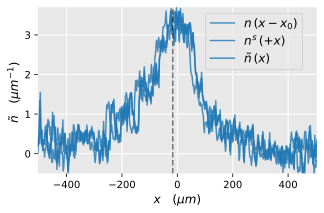
\includegraphics[width=0.5\textwidth]{Figures/article_asymetrie_24-04-2024}
    };
    \node[circle, draw=none, above=0cm of assy , shift={( -2.5cm , -0.5cm )}] {(b)};
\end{tikzpicture}
\caption{(a) {\it Profil de bord et tranche sélectionnée.} Le profil de bord après $18\,\mathrm{ms}$ est montré en jaune. L'ajustement thermique donne une température $T = 560\,\mathrm{nK}$ (orange). Le profil de densité mesuré $1\,\mathrm{ms}$ après la sélection de la tranche est en bleu. (b) {\it Asymétrie du profil d’expansion de la tranche.} Le profil de densité après une expansion pendant $\tau = 30\,\mathrm{ms}$ est comparé à son image miroir. Le centre de symétrie $x_s = -17\,\mu$m minimise la distance quadratique $\delta^2 = \int dx\, (\tilde{n}(x) - \tilde{n}(2x_s - x))^2$.}
\label{fig:simul_deformation}
\end{figure}

Pour aller au-delà de cette observation qualitative, nous effectuons un calcul GHD à l’échelle d’Euler du profil d’expansion, en supposant que l’état initial est thermique.  
La température est obtenue par ajustement du profil de bord avant la sélection de la tranche, comme indiqué en Fig.~\ref{fig:simul_deformation}(a), ce qui donne $T = 560$ nK.  
Le potentiel chimique est ajusté afin que la densité linéaire initiale corresponde à celle mesurée dans la région $x > 0$, avant l’élargissement du bord.  
À partir du profil initial, nous simulons à la fois l’élargissement du bord et l’expansion de la tranche en GHD, en supposant une découpe parfaite, c’est-à-dire $\nu(x,\theta) = 0$ pour $|x - x_0| > \ell/2$ et $\nu(x,\theta)$ inchangé sinon.  
La largeur $\ell$ est ajustée de sorte que le nombre d’atomes sélectionnés dans la simulation corresponde à celui mesuré expérimentalement après expansion, et on obtient $\ell = 24\,\mu$m.  

Le profil d’expansion simulé est montré en Fig.~\ref{fig:simul_expansion}(a).  
Il présente une forte asymétrie, comme attendu, avec un bord droit abrupt et une densité nulle au-delà d’un certain point.  
Cependant, cette chute est moins marquée que celle prédite pour la distribution locale des rapidités $\rho(x_0,\theta)$ à $x = x_0$. Deux effets contribuent à cet élargissement :  
(i) la distribution en rapidité n’est pas homogène à l’intérieur de la tranche, si bien que $\Pi(\theta)$ diffère de $\ell \rho(x_0,\theta)$, comme le montre la comparaison entre la ligne marron pleine et la ligne pointillée en Fig.~\ref{fig:simul_expansion}(a) ;  
(ii) le temps d’expansion est fini, de sorte que le profil observé ne correspond pas exactement à $\Pi((x-x_0)/\tau)/\tau$, comme le montre la comparaison entre les courbes marron et rouge.

\begin{figure}[!htb]
\centering
\begin{tikzpicture}
    \node[rectangle, draw = none] (exp) at (0,0) {
        %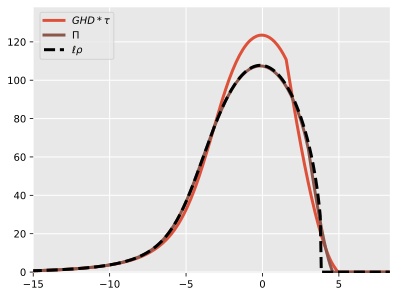
\includegraphics[width=0.5\textwidth]{Figures/article_distribution_24-04-2024}
    };
    \node[circle, draw=none, above=0cm of exp , shift={( -2.5cm , -0.5cm )} ] {(a)};
    
    \node[right=1mm of exp , shift={( -0.5cm , 0cm )}] (pi) {
        %\includegraphics[width=0.5\textwidth]{Figures/article_simul_expansion_1_24-04-2024-T-x0.pdf}
    };
    \node[circle, draw=none, above=0cm of pi , shift={( -2.5cm , -0.5cm )}] {(b)};
\end{tikzpicture}
\caption{(a) {\it Profil de densité après expansion de la tranche : effets de la largeur finie et du temps d’expansion fini.} Courbe orange : profil obtenu par simulation GHD après expansion pendant $\tau = 30$ ms, avec $T = 560$ nK. Courbe marron : distribution asymptotique $\Pi((x - x_0)/\tau)/\tau$. Courbe pointillée noire : approximation $\ell \rho(x_0, (x - x_0)/\tau)/\tau$ dans le cas d’une tranche étroite. (b) {\it Comparaison aux données expérimentales.} En bleu : profil expérimental après expansion pendant $\tau = 30$ ms. En orange : simulation GHD avec $T = 560$ nK. En magenta : ajustement du profil expérimental donnant $T = 1550$ nK.}
\label{fig:simul_expansion}
\end{figure}

Enfin, nous comparons le profil d’expansion simulé par GHD aux données expérimentales.  
Comme montré en Fig.~\ref{fig:simul_expansion}(b), le profil prédit reproduit les principales caractéristiques du profil observé expérimentalement.  
Des écarts allant jusqu’à 25\% sont néanmoins visibles dans la partie centrale.  
Afin d’améliorer la concordance, nous ajustons le profil d’expansion expérimental avec la simulation GHD en prenant la température initiale comme paramètre libre.  
Le résultat, représenté par la courbe magenta dans la Fig.~\ref{fig:simul_expansion}(b), ...

